%%notwendige packages

%----------------------------

\documentclass[12pt]{article}
%benötigt man immer
\usepackage{amsmath}
%is used for numbering of equations
\usepackage[english]{babel}
\usepackage[utf8x]{inputenc}
\usepackage{varwidth}
\usepackage{float}
% Table caption on top of tables
%\floatstyle{plaintop}
\restylefloat{table}
%----
\usepackage{makecell}
\usepackage{enumitem}

% Für fette Mathesymbole
\usepackage{amsfonts}
\usepackage{amsthm}
\usepackage{bm}
\renewcommand*{\mathbf}[1]{\ifmmode\bm{#1}\else\textbf{#1}\fi}
\usepackage{physics}


% Create links to references etc.. Usually with function autoref{}...
\usepackage{hyperref}


% For the type of citation and bibliographic style
%\usepackage{apacite}

% allows index generation
\usepackage{makeidx}
\makeindex

% equation, table and figure numbering should start with section number e.g. (3.1)
\numberwithin{equation}{section}
\numberwithin{table}{section}
\numberwithin{figure}{section}

%fonts
\usepackage[T1]{fontenc}

\usepackage{uarial}
\renewcommand{\familydefault}{\sfdefault}
\usepackage{blindtext}

\usepackage{textcomp}
%\usepackage{mathptmx}
\usepackage{tabularx}
\usepackage{multirow}
\usepackage{enumitem}
%small fonts for captions of figures and tables
\usepackage[center]{caption}
\captionsetup[figure]{font = footnotesize}
\captionsetup[table]{font = footnotesize}


%format
% Witwen und Waisenkinder vermeiden
\clubpenalty=4500	% Waisen vermeiden (erste Zeile eines neuen Absatzes als letzte Zeile einer Seite)
\widowpenalty=10000	% keine Witwen zulassen (letzte Zeile eines Absatzes am Beginn einer neuen Seite)

% Seitenraender einstellen
\usepackage{geometry}
\geometry{a4paper,left=30mm,right=30mm, top=20mm, bottom=20mm}

% Zeilenabstand
\linespread{1.5} 

% Disable indentation for the entire document
\setlength\parindent{0pt}

% turn off hyphenation and justification (Silbentrennung ausschalten)
\tolerance=1
\emergencystretch=\maxdimen
\hyphenpenalty=10000
\hbadness=10000

%Graphics
\usepackage[final]{graphicx} 	
\usepackage[twoside,figuresright]{rotating}
\usepackage{subcaption} 
%\usepackage{subfigure} 

% Adjust tables (and figures) to textwidth...
\usepackage{adjustbox}

%For tables, to color whole row without missing pieces...
\usepackage{tabularx}
%\usepackage[table]{xcolor}  % option loads »colortbl«

% Initialize Makro for table heads
\renewcommand\theadfont{\bfseries\sffamily}

% Highlighting rows, columns and headers of tables
\usepackage{color, colortbl}
\definecolor{Gray}{gray}{0.9}
\definecolor{LightCyan}{rgb}{0.88,1,1}
\definecolor{SeaBlue}{rgb}{0.3, 0.58, 1}

%acronym package for Abbreviations
\usepackage{acronym}
% macro for first letter capital (e.g. in new sentence)
%\usepackage{etoolbox}


%package to capitalize first letter in a word. Use function 
%\capitalisewords{first letter upper case}
%\usepackage{mfirstuc}

%Create Statutory Declaration page for signatures
\newcommand{\namesigdate}[2][3cm]{%
  \begin{tabular}{@{}p{#1}@{}}
    #2 \\[2\normalbaselineskip] \hrule \\[0pt]
    {\small \textit{Signature}}
  \end{tabular}
}

% Headers for the pages
%\usepackage{fancyhdr}
%\pagestyle{headings}

%\fancyhf{}

\usepackage{fancyhdr}
\pagestyle{fancy}
\fancyhf{}
\fancyhead[L]{\scriptsize \nouppercase{\leftmark}}
%\fancyhead[R]{\scriptsize \thepage}
\fancyfoot[C]{\thepage}
\renewcommand{\headrulewidth}{0.5pt}
% Hide section number in headnote
%\renewcommand\sectionmark[1]{\markboth{#1}{}}


%----------------------------

\begin{document}

\thispagestyle{empty}	
% !TEX root = Master.tex

%titlepage
\thispagestyle{empty}
\begin{center}


\begin{minipage}{0.75\linewidth}
    \centering
%University logo
    
\includegraphics[scale = 0.7]{figures/uni_goettingen_logo.eps}\\
    
    %\rule{0.4\linewidth}{0.15\linewidth}\par
    \vspace{1cm}
    
% Master Thesis
{{\Huge \textbf{Master Thesis} \par}}
    
\vspace{0.5cm}
    
%Thesis title
    {{\LARGE Multivariate Modelling of the Dependence Structure between Article Sales of a Sportswear Manufacturer\par}}
    \vspace{1cm}
    
    
%Author's name
\begin{center}
Author\\
{\LARGE \textbf{Petros Christanas}} \\
{\large petroschristanas@gmail.com}


\vspace{0.5cm}

Matriculation Number \\
{\large 11604278}

\vspace{1cm}

{\Large Applied Statistics M.Sc.}\\
{\large Chair of Statistics and Econometrics}

\end{center}
    
    \end{minipage}
\end{center}


\vspace{1.5cm}

\noindent Supervisors\\
\noindent {\Large \textbf{Prof. Dr. Thomas Kneib}} \\
\noindent {\Large \textbf{Dipl.-Vw. Quant. Fabian H. C. Raters}} \\

\vspace{0.5cm}
    
%Date
\begin{flushleft}
\noindent {\normalsize Submitted \today} \\
\noindent {\normalsize Processing time of 20 weeks}
\end{flushleft}

    
    

\clearpage


%\newpage
%\null\thispagestyle{empty}
%\newpage
%\thispagestyle{empty}
%\section*{Confidentiality Clause}
%\input{confidentiality_clause}

%\clearpage
%\newpage
%\null\thispagestyle{empty}
%\newpage
%\thispagestyle{empty}
%\section*{Statutory Declaration}
%\input{statutory_declaration}



%\newpage
%\null\thispagestyle{empty}
%\newpage
%\thispagestyle{empty}
%\section*{Acknowledgments}
%\input{acknowledgments}
%\newpage
%\null\thispagestyle{empty}
%\newpage


	
%\pagenumbering{Roman} 	
\thispagestyle{empty}
\tableofcontents
\newpage




\newpage

\pagenumbering{arabic} 
\setcounter{page}{1} 

\section{Introduction} \label{sec:introduction}
\input{introduction}
\subsection{Data Sources} \label{ssec:data_sources}
% !TEX root = Master.tex

Throughout each season, transactional data are collected from online purchases of the sports brand's e-Commerce website. Specifically, weekly sales data for western European countries consisting of 109 observed weeks in total are provided. A short description is depicted in \autoref{tab:transactional_data}.\\

\begin{table}[H]
\setlength\arrayrulewidth{1pt}  
\centering
\begin{adjustbox}{max width=\textwidth}
\begin{tabular}{|l|l|l|}
\hline
\rowcolor{lightgray} 
\textbf{Column}         & \textbf{Description}                                                                                                        & \textbf{Values}              \\ \hline
week\_id                & Calender week of a specific year (YYYYWW)                                                                         & Factors:\textit{ 201648, ..., 201852}          \\ \hline
article\_number         & Unique article identification number (article ID)                                                                           & Factors: \textit{10669, 10, ...       }        \\ \hline
min\_date\_of\_week     & \begin{tabular}[c]{@{}l@{}} Minimum date of the respective week; always a Monday \\ (YYYY-MM-DD)                                                          \end{tabular} & Dates: \textit{2016-11-28, ..., 2018-12-24}  \\ \hline
art\_min\_price         & Minimal recorded price of the article                                                                                       & Non-negative (integer) value \\ \hline
month\_id               & Calender month of a specific year (YYYYMM)                                                                               & Factors: \textit{201612, ..., 201812}          \\ \hline
season                  & \begin{tabular}[c]{@{}l@{}}Season of year (format: SSYY) \\ (Spring-Summer [SS]:  December - May)\\  Fall-Winter [FW]: June - November)\end{tabular} & \begin{tabular}[c]{@{}l@{}}  Factors: \\ \textit{SS17, FW17,} \\\textit{ SS18, FW18, SS19} \end{tabular} \\

 \hline
bf\_w                   & Weekly "Black Friday" promotion intensity of the article                                                                    & Between \textit{0} and \textit{1}              \\ \hline
ff\_w                   & Weekly "Friends \& Family" promotion intensity of the article                                                               & Between \textit{0} and \textit{1}              \\ \hline
ot\_w                   & Weekly article promotion intensity of "Other" type                                                                          & Between \textit{0} and \textit{1}              \\ \hline
gross\_demand\_quantity & Weekly amount of added articles to shopping cart                                                                            & Non-negative (integer) value \\ \hline
base\_price\_locf       & Retail price of the article without any discounts                                                                           & Non-negative (integer) value \\ \hline
total\_markdown\_pct    &                                                                                                          Total markdown percentage of the article &    Non-negative                           \\ \hline
day\_of\_month          & Day of the month                                                                                                            & Integers: \textit{1 - 31}                       \\ \hline
month\_of\_year         & Month of the year                                                                                                           & Factors: \textit{January, ..., December}       \\ \hline
year                    & Year                                                                                                                        & Integers: \textit{2016, 2017, 2018}             \\ \hline
week\_of\_year          & Week of the year                                                                                                            & Integers: \textit{1 - 52}                       \\ \hline
\end{tabular}
\end{adjustbox}
\caption{Transactional raw data description from online purchases of western European countries}
\label{tab:transactional_data}
\end{table}

Due to legal regulations of the company, some columns had to undergo anonymization in order for the data to be released. To ensure data protection and confidentiality, numeric variables (with exception of time-indicating columns) were transformed. As a consequence for the analysis part, most integer values were converted to float numbers. This fact should be kept in mind by the reader, since the above table serves as a reminder and reference point for the data documentation.\\

Another peculiarity of this setup is to be considered, too. We will often refer to the variable \textit{gross demand quantity} as \textit{sales}, even though it is obviously not exactly the same. In the e-Commerce environment, there are several stages before the purchase is complete, e.g. addition to cart, removal from cart, proceeding to checkout \& even the return of bought articles. Targeting the articles added to cart, i.e. the (gross) demand quantity, provides the optimal data extraction for analytical purposes and is the closest to adequately model the dependence structure between net sales of articles.\footnote{Gross demand quantity will be our target as we follow the adidas norm}  \\

Besides the transactional data, attributes of the articles are provided and described in \autoref{tab:article_master_data}. Some attributes of special importance will be explained in more detail later on in Chapter \ref{sec:data_exploration}. \\

\begin{table}[H]
\setlength\arrayrulewidth{1pt}  
\centering
\begin{adjustbox}{max width=\textwidth}
\begin{tabular}{|l|l|l|}
\hline
\rowcolor{lightgray}
\textbf{Column}           & \textbf{Description}                                   & \textbf{Values (all Factors)}                 \\ \hline
article\_number           & Unique article identification number (article ID)      & \textit{10669, 10, ...}                                \\ \hline
gender                    & Gender type of the article (Men, Women, Unisex)        & \textit{M, W, U}                                       \\ \hline
age\_group                & Age group of the article (Adult, Infant, Junior, Kids) & \textit{A, I, J, K}                                    \\ \hline
key\_category\_descr      & Key category of the article & \textit{KC\_1, ..., KC\_15}   \\ \hline
key\_category\_cluster\_descr      & Key category cluster of the article & \textit{KCC\_1, ..., KCC\_9}   \\ \hline
product\_division\_descr  & Product division of the article                        & \textit{Apparel, Footwear, Hardware}                   \\ \hline
product\_group\_descr     & Product group of the article                           & \textit{Bags, Balls, Footwear Accessories, Shoes, ...} \\ \hline
color                     & Consolidated color group of the article                & \textit{Beige, Black, Brown, Orange, Pink, Red, ... }  \\ \hline
sports\_category\_descr   & Sports category of the article                         & encoded: \textit{SC\_1, ..., SC\_22 }                  \\ \hline
sales\_line\_descr        & Sales line of the article                              & encoded: \textit{SL\_1, ..., SL\_379 }                 \\ \hline
business\_unit\_descr     & The article's Business Unit membership                 & encoded:\textit{ BU\_1, ..., BU\_18   }                \\ \hline
business\_segment\_descr  & The article's Business Segment membership              & encoded: \textit{BS\_1, ..., BS\_49  }                 \\ \hline
sub\_brand\_descr         & Sub-brand of the article                               & encoded: \textit{sub-brand\_1, ..., sub-brand\_4 }     \\ \hline
item\_type                & Item type of the article                               & encoded: \textit{IT\_1, ..., IT\_171 }                 \\ \hline
brand\_element            & Brand element of the article                           & encoded: \textit{BE\_1, ..., BE\_131 }                   \\ \hline
product\_franchise\_descr & Product franchise of the article                       & encoded: \textit{franchise\_1, ..., franchise\_72}     \\ \hline
product\_line\_descr      & Product line of the article                            & encoded: \textit{PL\_1, ..., PL\_105 }                 \\ \hline
franchise\_bin            & Franchise indicator of the article                     &\textit{Franchise, Non-Franchise }                     \\ \hline
category                  & Category of the article                                & encoded: \textit{category\_1, category\_2}             \\ \hline
\end{tabular}
\end{adjustbox}
\caption{Article attribute data}
\label{tab:article_master_data}
\end{table}

%Plenty of additional information is stored in the database, but we are %neglecting columns omitted in these tables, as they are redundant, %already summarized, transformed or simply do not provide any value.\\
Overall, these are the primary data sources and we will be working with data collected over two years, namely the years 2017 and 2018, while some transactions of late 2016 are attached marginally. In summary, after joining the transactional observations to the article attributes by the article ID, this translates to a dataset of 587,127 instances including 26,203 distinct articles and over 30 variables. 


\clearpage

\section{Statistical Theory \& Methods} \label{sec:theory_and_methods}
% !TEX root = Master.tex

This chapter introduces some statistical methods used during the conduction of this thesis. Basic notations regarding mathematical foundations of statistics (such as linear algebra, probability theory, hypothesis testing etc) are skipped. Theoretical aspects regarding copulas and dependence structures will be introduced separately in Chapter \ref{sec:copulas_and_dependence_structures}.
%The chapter starts off with some fundamental notions on generalized linear models and arrives at a brief introduction to additive models


\subsection{Generalized Linear Models} \label{ssec:glm}
% !TEX root = Master.tex
\textit{\acp{GLM}} are an extension of the classical \textit{\ac{LM}}
\begin{equation}
\begin{aligned}
&y_{i}=\beta_{0}+\beta_{1} x_{i 1}+\ldots+\beta_{k} x_{i k}+\varepsilon_{i}, &i=1, \ldots, n
\end{aligned}
\end{equation}
which in matrix notation can be written as
\begin{equation}
 \bm{y} = \bm{X}\bm{\beta} + \bm{\epsilon} 
\end{equation}
where the response variable $y_i$ can take values from several probability distributions (e.g. Poisson, Binomial, Gamma, ...), which are members of the exponential family \citep{fahrmeir2003regression}. The linear predictor 
\begin{equation} 
\eta_i = \beta_{0}+\beta_{1} x_{i 1}+\ldots+\beta_{k} x_{i k}+\varepsilon_{i} = \bm{x'}_i \bm{\beta} + \bm{\varepsilon}
\label{eq:linear_predictor_glm}
\end{equation}
is passed through a \textit{response function h} (a one-to-one, twice differentiable transformation), such that
\begin{equation}
 E(y_i) = h(\eta_i),
\label{eq:response_function}
\end{equation}
where $h$ ensures that the expected value of the response variable belongs to the appropriate value range. The inverse of the response function, i.e.
\begin{equation}
g = h^{-1},
\label{eq:link_function}
\end{equation} 
is called the \textit{link function} and transforms the mean of the response's distribution to an unbounded continuous scale.

% MAXIMUM LIKELIHOOD ESTIMATION HERE??...




\subsection{Generalized Additive Models} \label{sec:gam}
%input{gam}
\subsection{Mixed Effects Models} \label{ssec:mixed_models}
% !TEX root = Master.tex
The \textit{\ac{LMM}} is powerful tool when dealing with clustered data or data with a longitudinal structure (repeated measurements of individuals).
As in the classical \acs{LM}, there are population-specific effects, namely the parameter vector of \textit{fixed effects} $\boldsymbol{\beta}$, as well as the cluster- or individual-specific effects of such models called \textit{random effects} \cite{fahrmeir2003regression}. In the following, we will refer to our clusters or individuals as "groups" for briefness.\ Mathematically speaking, the linear predictor $\eta_{ij}= \mathbf{x}'_{ij} \mathbf{\beta} $ is extended to
\begin{equation}
\eta_{ij} = \bm{{x'}}_{ij} \bm{\beta} + \bm{u'}_{ij}\bm{\gamma}_i, \quad j=1, \ldots, m, \quad i=1, \ldots, n_i, 
\label{eq:linear_mixed_predictor}
\end{equation}
where
\begin{itemize}
\item $i$ is the number of groups
\item $j$ is the number of observations per group
\item $\bm{\beta}$ is the vector of fixed effects
\item $\bm{\gamma}_i$ is the vector of random effects
\item $\bm{x'}_{ij}$ is the vector of covariates and
\item $\bm{u'}_{ij}$ is a subvector of $\bm{x'}_{ij}$.
\end{itemize}


$\bm{x'}_{ij} = (1, x_{ij1}, \ldots, x_{ijk}) $ and $ \bm{u'}_{ij} = (1, u_{ij1}, \ldots, u_{ijk}) $ are therefore the design vectors and $\varepsilon_{ij}$ are the error terms of the \textit{measurement model}

\begin{equation}
y_{ij} =  \bm{x'}_{ij} \bm{\beta} + \bm{u'}_{ij} \bm{\gamma}_i + \epsilon_{ij}, \quad \varepsilon_{i j} \overset{i.i.d.} \sim N\left(0, \sigma^{2}\right) 
\end{equation}
or in matrix notation

\begin{equation}
\bm{y}_{i}=\bm{X}_{i} \bm{\beta} + \bm{U}_{i} \bm{\gamma}_{i} + \bm{\varepsilon}_{i}
\end{equation}
for group $ i=1, \ldots, m $ with $ E(\bm{\varepsilon}_{i}) = \bm{0}$. \\

Similar to \ac{GLM}s, the \textit{\ac{GLMM}} relates the linear mixed predictor \ref{eq:linear_mixed_predictor} to the conditional mean 
$ \mu_{ij} = E(y_{ij} | \bm{\gamma}_{i}) $
via a suitable response function $h$, such that
$ \mu_{ij} = h(\eta_{ij}) $ and thus the conditional density of $y_{ij}$ belongs to the exponential family.
%\input{random_intercept_model}
\clearpage

\section{Copulas \& Dependence Modelling} \label{sec:copulas_and_dependence_moelling}
% !TEX root = Master.tex

Multivariate distributions consist of the marginal distributions and the dependence structure between those marginals. These components can be specified separately in a single framework with the help of copula functions. This chapter introduces the concept of modelling such dependency structures with copulas, which is the main focus of this thesis.
\subsection{Introduction to Copulas} \label{ssec:intro_to_copulas}
% !TEX root = Master.tex

A $d$-dimensional function $C: [0,1]^d \rightarrow [0,1]$ is called a \textit{copula}, if it is a \ac{CDF} with uniform margins, i.e.
\begin{equation*}
P\left(U_{1} \leq u_{1}, \ldots, U_{d} \leq u_{d}\right)=C\left(u_{1}, \ldots, u_{d}\right)
\end{equation*}
where 
$ U_{i}, \hspace{0.25em} i = 1, \ldots, d $ 
are uniformly distributed \acp{RV} in $[0,1]$.\\

\textbf{Probability Transformation}\\
If a \ac{RV} $Y$ has a continuous \ac{CDF} $F$, then
\begin{equation}
F(Y) \sim U[0,1].
\label{eq:probability_transformation}
\end{equation}

\hfill $\square$ \\

The reverse of the \textit{probability transformation} is the \textit{quantile transformation}.\\

\textbf{Quantile Transformation}\\
If $U \sim U[0,1]$ and $F$ be a \ac{CDF}, then
\begin{equation}
P\left(F^{-1}(U) \leq x\right)=F(x)
\label{eq:quantile_transformation}
\end{equation}

\hfill $\square$ \\

The above two transformations allow us to move back and forth between $\mathbb{R}^d$ and $[0,1]^d$ and are the primary building blocks regarding copulas. Against this backdrop, we introduce \textit{Sklar's theorem} which is considered the foundation of all copula related applications.\\




\textbf{Sklar's Theorem} \cite{sklar1959fonctions} \\
Let $F$ be a $d$-dimensional \ac{CDF} with marginal distributions $F_{i}, \hspace{0.25em} i = 1, \ldots, d$.
Then there exists a copula $C$ such that
\begin{equation}
F(x_1, \ldots, x_d) = C (F_1(x_1), \ldots, F_d(x_d))
\label{eq:sklar}
\end{equation}
for all $x_i \in \mathbb{R}, \hspace{0.25em} i = 1, \ldots, d $.\\
The copula $C$ is unique, if $ \hspace{0.25em} \forall i = 1, \ldots, d \hspace{0.25em}$,  $F_i \hspace{0.25em}$  is continuous. Otherwise $C$ is uniquely determined only on
$Ran(F_1) \times \ldots \times Ran(F_d)$, where $Ran(F_{i})$ is the range of $F_i$.\\
Conversely, if $C$ is a $d$-dimensional copula and $F_1, \ldots, F_d$ are univariate \ac{CDF}'s, then $F$ as defined in \autoref{eq:sklar} is a 
$d$-dimensional \ac{CDF}.

\hfill $\square$ \\


If the copula has a \ac{PDF}, then the \textit{copula density} is defined as
\begin{equation}
c(\mathbf{u})=\frac{\partial^{d} C\left(u_{1}, \ldots, u_{d}\right)}{\partial u_{1} \cdots \partial u_{d}} 
\label{eq:copula_density_1}
\end{equation}
for a differentiable copula function $C$ and the realization of a random vector $ \bm{u} = (u_1, \ldots, u_d)$.\\

By virtue of \autoref{eq:sklar} in Sklar's theorem and given that
\begin{equation} 
C(\mathbf{u})=F\left(F_{1}^{-1}\left(u_{1}\right), \ldots, F_{d}^{-1}\left(u_{d}\right)\right) ,
\label{eq:sklar_inverse}
\end{equation}
i.e. inversible \ac{CDF}s $ F_i, \hspace{0.25em} i = 1, \ldots, d, \hspace{0.25em}$ we can rewrite the copula density to
\begin{equation}
c\left(u_{1}, \ldots, u_{d}\right)=\frac{f\left(F_{1}^{-1}\left(u_{1}\right), \ldots, F_{d}^{-1}\left(u_{d}\right)\right)}{\prod \limits _{i=1}^{d} f_{i}\left(F_{i}^{-1}\left(u_{i}\right)\right)}
\label{eq:copula_density_2}
\end{equation}
for densities $f$ of $F$ and $f_1, \ldots, f_d$ of the corresponding marginals.\\


\textbf{Invariance Principal}\\
Suppose the \ac{RV}s $ X_1, \ldots, X_d $  have continuous marginals and copula $C$. For strictly increasing functions $T_i : \mathbb{R} \rightarrow \mathbb{R}, i = 1, \ldots, d$, the \ac{RV}s $T_1(X_1), \ldots, T_d(X_d)$ also have copula $C$.

\hfill $\square$ \\


\textbf{Fr\'echet-Hoeffding Bounds}\\
Let $C(\bm{u}) = C(u_1, \ldots, u_d)$ be any $d$-dimensional copula.\\
Then, for
\begin{equation}
W(\boldsymbol{u})=\max \left\{\sum\limits_{i=1}^{d} u_{i}-d+1, \hspace{0.25em} 0\right\}
\label{eq:frechet_hoeffding_lower}
\end{equation}
as well as
\begin{equation}
M(\boldsymbol{u})=\min \limits _{1 \leq i \leq d}\left\{u_{i}\right\},
\label{eq:frechet_hoeffding_upper}
\end{equation}
it holds that
\begin{equation}
W(\bm{u}) \leq C(\bm{u}) \leq M(\bm{u}), \quad \bm{u} \in[0,1]^{d}.
\label{eq:frechet_hoeffding}
\end{equation}\\
We call $W$ the \textit{lower Fr\'echet-Hoeffding bound} and $M$ the \textit{upper Fr\'echet-Hoeffding bound}.\\
Note that $W$ is a copula if and only if $d=2$, whereas $M$ is a copula for all $d \geq 2$ (more on this later in Section \ref{sssec:fundamental_copulas}).

\hfill $\square$ \\


MORE ON COPULA THEORY (NOTES)




\subsection{Copula Classes} \label{ssec:copula_classes}
% !TEX root = Master.tex

In this section we will take a look at three very popular \textit{copula classes}, namely \textit{fundamental, elliptical and archimedean copulas}. For each class, a few (parametric) \textit{copula families}, which are widely used, will be presented.
\subsubsection{Fundamental Copulas} \label{sssec:fundamental_copulas}
% !TEX root = Master.tex

Fundamental copulas are a basic class of copulas, which emerge directly from the copula framework and do not depend on any parametric components. \\

\textbf{Independence Copula}\\
It is well known that the joint \ac{CDF} of a finite set of \acp{RV}
$X_i, i = 1, \ldots, n$, is equal to the product of the margins if and only if the \acp{RV} $X_i$ are mutually independent, i.e.
\begin{equation}
F_{X_{1}, \ldots, X_{n}}\left(x_{1}, \ldots, x_{n}\right)= \prod_{i=1}^{n} F_{X_{i}}\left(x_{i}\right)) \quad \forall x_1, \ldots, x_n.
\end{equation}

Equally, the exact same concept applies when we talk about the \textit{independence copula}, i.e.
\begin{equation}
\Pi (\bm{u}) = \prod \limits _{i = 1}^d u_i.
\end{equation}
As a result of Sklar's theorem, the \ac{RV}s $u_i$ are independent if and only if their copula is the independence copula, i.e.
\begin{equation}
 C(\bm{u}) = \Pi (\bm{u}) 
 \end{equation}
and thus the copula density would be 
\begin{equation}
c(\boldsymbol{u})=1, \quad \boldsymbol{u} \in[0,1]^{d}.
\end{equation}

%From \autoref{eq:frechet_hoeffding}, it is obvious that the Fr\'echet-Hoeffding bounds correspond to the extreme cases of perfect dependence between the \ac{RV}s $X_i, i = 1, \ldots, d$. \\

%\textbf{Comonotonicity Copula}\\
%Consider the \ac{RV}s $X_1, \ldots, X_d$ and strictly increasing transformations $T_1, \ldots, T_d$ and $X_i = T(X_i)$ for $i = 2, \ldots, d$. Making use of the \textit{invariance principal}, it can be shown that these \ac{RV}s have as copula the upper Fr\'echet-Hoeffding bound 
%$$M(\bm{u}) = \min\{ u_1, \ldots, u_d \}.$$ Since there is perfect positive dependence between those \ac{RV}s, $M$ is called the \textit{comonotonicity copula}. The number of dimensions $d$ can be any finite number greater than or equal to $2$ for $M$ to be a copula, as the minimum remains well defined.
%
%
%
%
%\textbf{Countermonotonicity Copula}\\
%Similar to the comonotonic case, it can be shown that if two \acp{RV} $X_1$ and $X_2$ are perfectly negatively dependent, their copula is the lower Fr\'echet-Hoeffding bound
%$$
%W(\boldsymbol{u})=\max \left\{\sum\limits_{i=1}^{d} u_{i}-d+1, \hspace{0.25em} 0\right\}.
%$$
%Therefore, $W$ is known as the \textit{countermonotonicity copula}. Because of the fact that countermonotonicity is not valid for a dimension greater than $2$, we end up with the restriction $d=2$ for $W$ to be indeed a copula.









\subsubsection{Elliptical Copulas} \label{sssec:elliptical_copulas}
% !TEX root = Master.tex

Copulas which can be derived from known multivariate distributions like for example the \textit{Multivariate Normal (or Gaussian) Distribution} or the \textit{Multivariate Student's t-Distribution} are called \textit{implicit copulas}. \textit{Elliptical copulas} are implicit copulas which arise via Sklar's theorem from elliptical distributions like the mentioned examples.\\

\textbf{Gaussian Copula}\\
Without loss of generality, for a random vector $\bm{X} \sim {\mathcal{N}_{d}(\bm{0}, \mathbf{P})} $ and \textit{correlation matrix} $\bm{P}$,
the \textit{Gaussian copula (family)} is given by
\begin{equation}
C_{\mathbf{P}}^{G a}(\mathbf{u})=\Phi_{\mathbf{P}}\left(\Phi^{-1}\left(u_{1}\right), \ldots, \Phi^{-1}\left(u_{d}\right)\right),
\end{equation}
where $\Phi$ is the \ac{CDF} of $\mathcal{N}(0, \sigma^{2})$ and 
$\Phi_{\bm{P}}$ is the \ac{CDF} of $\mathcal{N}_{d}(\bm{0}, \mathbf{P})$.\\
There are special cases to this copula family, namely for $d=2$ and correlation $\rho$, the \textit{bivariate Gaussian copula} $C_{\rho}^{G a}$ is equivalent to
\begin{itemize}
\item the independence copula $\Pi$ if $\rho = 0$,
\item the comonotonicity copula $M$ if $\rho = 1$ and
\item the countermonotonicity copula $W$ if $\rho = -1$
\end{itemize}
The density of the Gaussian copula is given by
\begin{equation}
c_{\bm{P}}^{\mathrm{Ga}}(\boldsymbol{u})=\frac{1}{\sqrt{\operatorname{det} \bm{P}}} \exp \left(-\frac{1}{2} \boldsymbol{x}^{\prime}\left(\bm{P}^{-1}-\bm{I}_{d}\right) \boldsymbol{x}\right),
\end{equation}
where $\bm{x} = \left(\Phi^{-1}\left(u_{1}\right), \ldots, \Phi^{-1}\left(u_{d}\right)\right)$.

\hfill $\square$ \\




 \begin{figure}[H]
\centering
\begin{subfigure}{.45\textwidth}
  \centering
  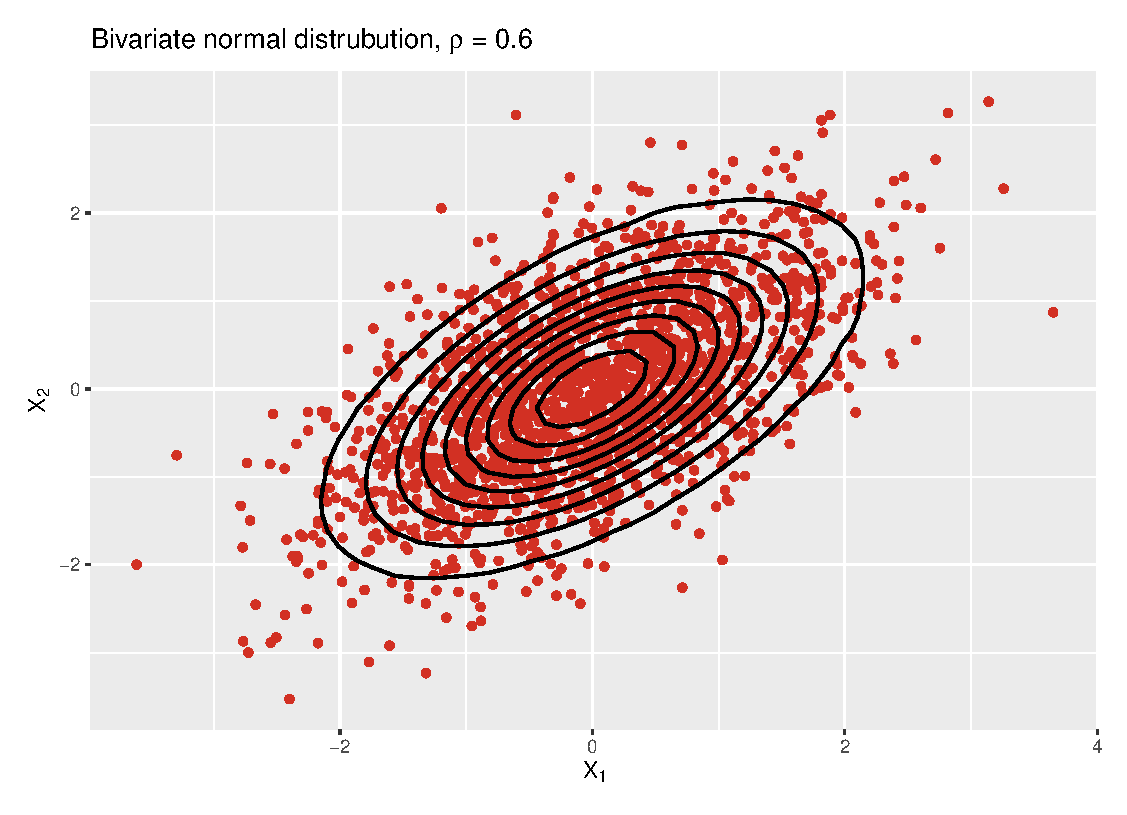
\includegraphics[width=\linewidth]{figures/bivariate_normal.eps}
  \caption{Gaussian distribution with contour lines}
  \label{fig:mvd_normal_copula}
\end{subfigure}
\begin{subfigure}{.45\textwidth}
  \centering
  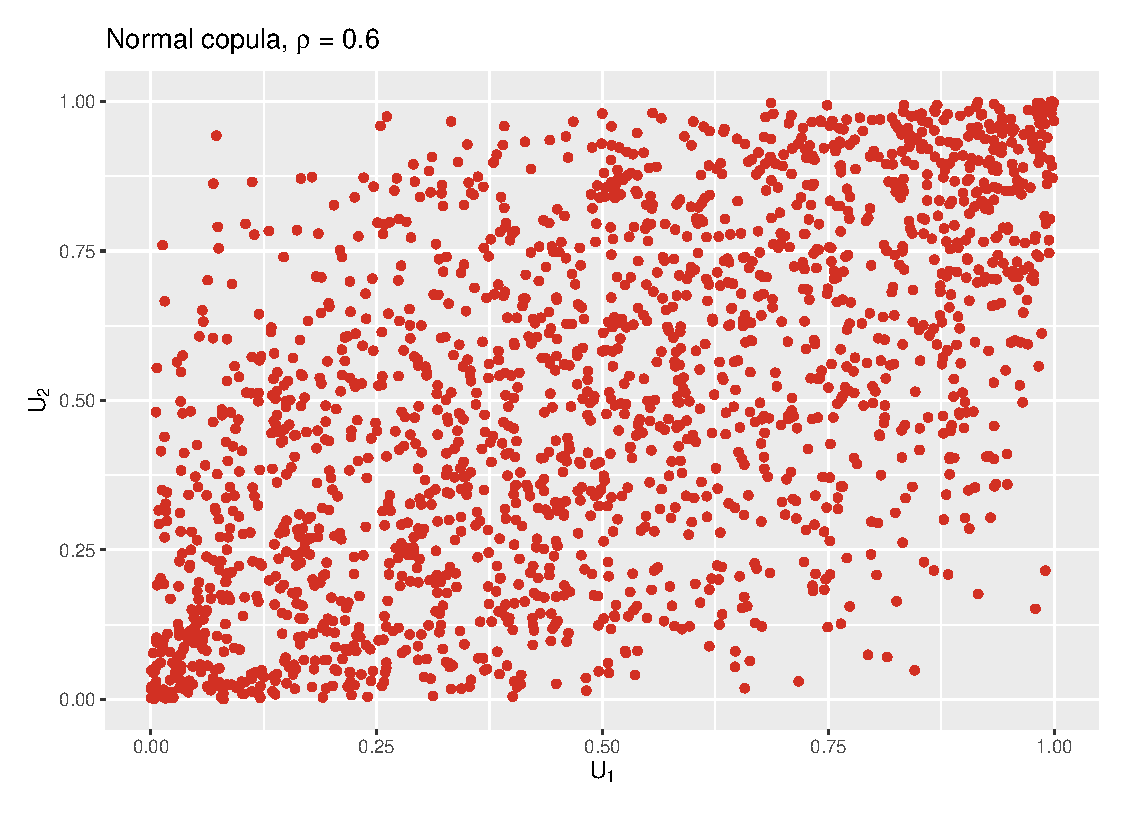
\includegraphics[width=\linewidth]{figures/normal_copula.eps}
  \caption{Gaussian copula}
  \label{fig:normal_copula}
\end{subfigure}
\caption{Bivariate Gaussian distribution and Gaussian copula for Pearson's $\rho = 0.6$ and simulated sample of size $n = 1800$, both with standard normal marginals}
\label{fig:normal_plots}
\end{figure}






\textbf{t-Copula}\\
Consider without loss of generality $\bm{X} \sim {t_{d}(\nu, \bm{0}, \mathbf{P})}$ (multivariate Student's t-distribution) with $\nu$ \ac{dof} and $\bm{P}$ a correlation matrix, then the \textit{t-copula (family)} is given by
\begin{equation}
C_{\nu, \bm{P}}^{t}(\mathbf{u})=t_{\nu, \bm{P}}\left(t_{\nu}^{-1}\left(u_{1}\right), \ldots, t_{\nu}^{-1}\left(u_{d}\right)\right),
\end{equation}
where $t_{\nu}$ is the \ac{CDF} of the univariate Student's t-distribution  and $t_{\nu, \bm{P}}$ is the \ac{CDF} of the multivariate Student's t-distribution (both with $\nu$ \ac{dof}).\\
For the \textit{bivariate t-copula} ($d=2$), the special cases are the same as for the Gaussian copula except that $d=0$ does not yield the independence copula (unless $\nu \rightarrow \infty$ in which case  $ C_{\nu, \rho}^{t} = C_{\rho}^{G a}$).\\
The density of $C_{\nu, \bm{P}}^{t}$ is given by
\begin{equation}
c_{\nu, \mathbf{P}}^{t}(\boldsymbol{u})=\frac{\Gamma((\nu+d) / 2)}{\Gamma(\nu / 2) \sqrt{\operatorname{det} \mathbf{P}}}\left(\frac{\Gamma(\nu / 2)}{\Gamma((\nu+1) / 2)}\right)^{d} \frac{\left(1+\boldsymbol{x}^{\prime} \mathbf{P}^{-1} \boldsymbol{x} / \nu\right)^{-(\nu+d) / 2}}{\prod_{j=1}^{d}\left(1+x_{j}^{2} / \nu\right)^{-(\nu+1) / 2}},
\end{equation}
where $\bm{x} = \left(t_{\nu}^{-1}\left(u_{1}\right), \ldots, t_{\nu}^{-1}\left(u_{d}\right)\right)$.

\hfill $\square$ \\






 \begin{figure}[H]
\centering
\begin{subfigure}{.45\textwidth}
  \centering
  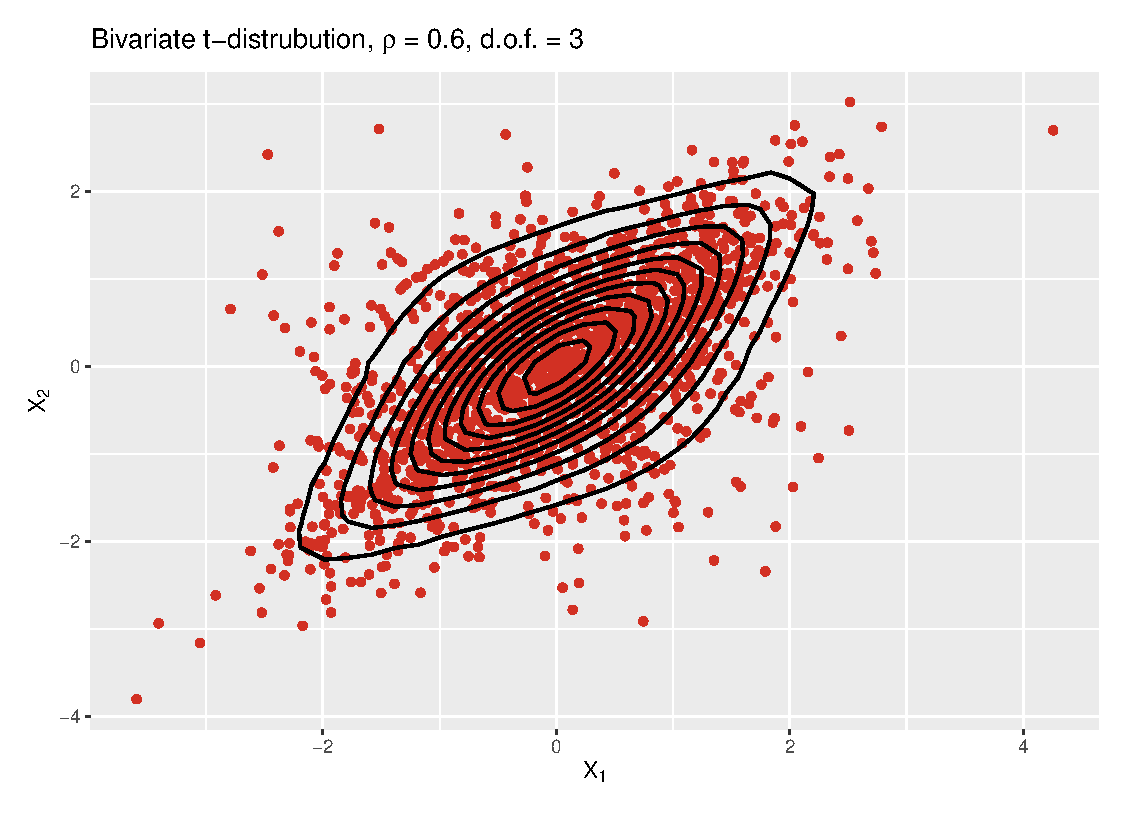
\includegraphics[width=\linewidth]{figures/bivariate_t.eps}
  \caption{t-distribution with contour lines}
  \label{fig:bivariate_t}
\end{subfigure}
\begin{subfigure}{.45\textwidth}
  \centering
  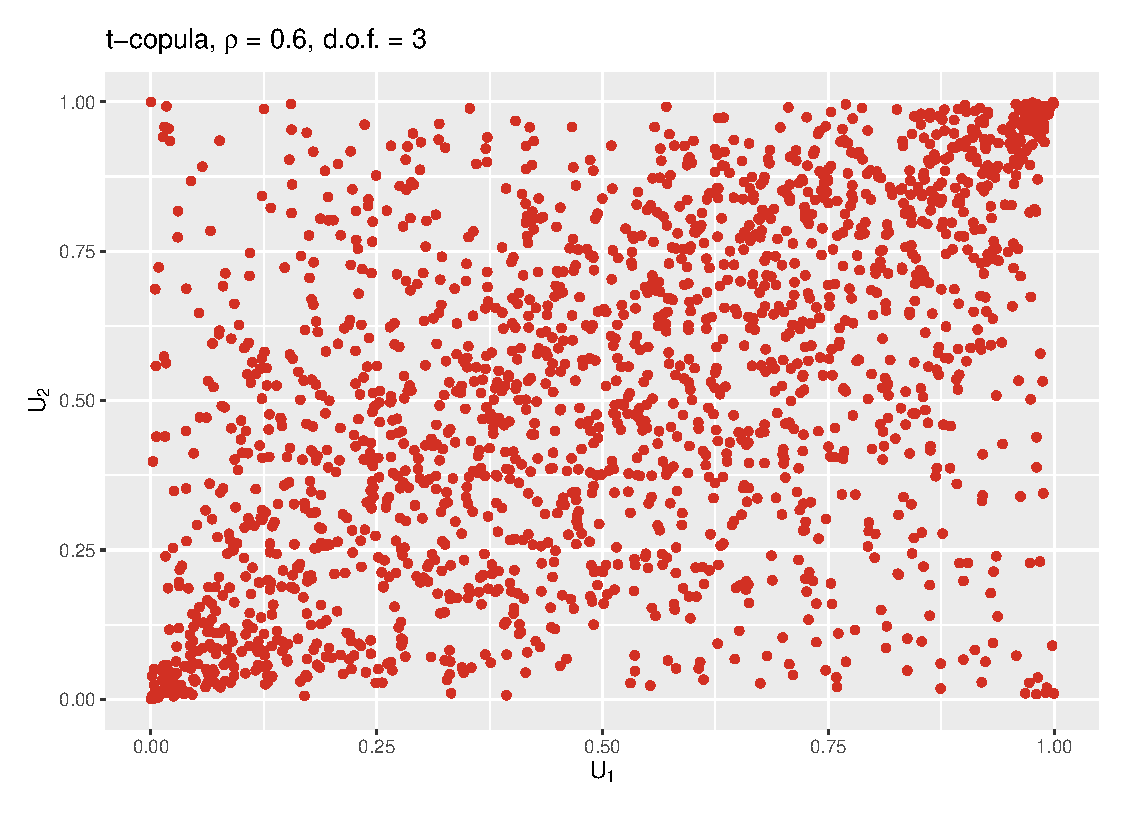
\includegraphics[width=\linewidth]{figures/t_copula.eps}
  \caption{t-copula}
  \label{fig:t_copula}
\end{subfigure}
\caption{Bivariate t-distribution and t-copula with 3 degrees of freedom for Pearson's $\rho = 0.6$ and simulated sample of size $n = 1800$, both with standard normal marginals}
\label{fig:t_plots}
\end{figure}







\subsubsection{Archimedean Copulas} \label{sssec:archimedean_copulas}
% !TEX root = Master.tex

Unlike implicit copulas, \textit{explicit copulas} can be specified directly by taking into account certain constructional principles. The most important aspects of a such explicit copulas, in particular \textit{archimedean copulas}, are showcased in this subsection. Archimedian copulas are of the general form
\begin{equation}C(\boldsymbol{u})=\psi\left(\psi^{-1}\left(u_{1}\right)+\cdots+\psi^{-1}\left(u_{d}\right)\right),
\label{eq:archimedean_generator}
\end{equation}
where the function $\psi:[0, \infty) \rightarrow[0,1]$ is the \textit{(archimedean) generator} and satisfies the following properties:
\begin{itemize}
\item $\psi$ is strictly decreasing in the entire domain $[0, \infty)$
\item $\psi (0) = 1$
\item $\psi(\infty)=\lim \limits _{t \rightarrow \infty} \psi(t)=0$
\item We set $\psi^{-1}(0)=\inf \{t: \psi(t)=0\}$
\end{itemize}
If $\psi(t)>0, t \in[0, \infty)$, we call $\psi$ \textit{strict}. The set of all generators is denoted by $\Psi$.\\
Based on \autoref{eq:archimedean_generator} and the generator, we can construct several copula families. Three of the most popular ones are the \textit{Gumbel}, the \textit{Clayton} and the \textit{Frank} \textit{copula}.





\subsection{Dependence Measures} \label{dependence_measures}
%input{dependence_measures}



\clearpage





%\section{Conclusion} 
%% !TEX root = Master.tex

The objective of this study is to contribute to the development of LiDAR assisted forest inventories by developing
a statistical sound approach to derive unbiased diameter distribution models from LiDAR data for homogeneous
compartments of the forest. Prediction is successfully performed by a generalized linear
regression model using the gamma distribution with log as a link function. Clustering the compartments into three groups led to enough samples per cluster to
perform distribution engineering. Clustering is not meant to find groups upon a decision for more or less correction is made, but
to find an appropriate correction for similar compartments. Clustering further uncovered the issue of not detecting
equally height trees, which introduced additional bias in the tree diameter prediction. Bias correction is
achieved by fitting a gamma distribution on the diameter distribution of each cluster from the inventory dataset
and subsequently the predicted diameter distribution. A correction factor is calculated based on the ratio of the
shape and scale parameter of both fitted distributions for each cluster. High confidence is thus given to the
inventory dataset. Subsequently, the correction factor is applied for each section. \\

This approach could solve all present challenges, without relying on any heuristic methods apart from choosing
an appropriate amount of clusters and variables. Hence the objective of finding a statistical sound approach is achieved.\\

We could not find studies with similar approaches to the objective. 
The achieved residual standard error of the mean diameter of the corrected compartment distribution of 5.49cm (see Section \ref{Results}) is satisfying.
To compare and assess the modelling of the distribution, a inventory dataset of fully sampled compartments is necessary. 
The RSE could be further reduced by improving the tree species detection rate and likely crown area estimation. Comparing different amount of k cluster could be an interesting extension. 
The residual standard error of the regression model with 3.81cm is compared to another study. G. Liu, J. Wang, P. Dong, Y. Chen, Z. Liu (2018) [17] achieved a significantly better diameter residual standard error of 1.28 cm using solely LiDAR data. \textit{"Octree segmentation, connected component labelling and random Hough transform are comprehensively used to identify trunks and extract DBH of trees in sample plots."} \\

Nevertheless, this sophisticated approach can only be applied on plot level (small sampling location in a forest) and likely not scaled up on a whole forest. Ultimately, a residual standard error of below 5cm is satisfying. \\

The advantage of the presented approach is that an extension of the estimation of the unbiased tree diameter distribution based on just the LiDAR scanning system can be achieved, even though the majority of the area did not undergo any manual sampling activities.\\
Additionally, by making use of this bias correction attempt by fitting and adjusting parametric distributions instead of just relying on the predicted diameter distribution, outlier occurrences at the outer quantiles are no longer an issue (due to overestimated crown areas), meaning that overestimation of the tree diameter is also prevented. 




%\clearpage


\fancyhead[L]{\scriptsize Appendix}
\addcontentsline{toc}{section}{Appendix}
\section*{Appendix} \label{sec:appendix}
\input{appendix}
\clearpage


\fancyhead[L]{\scriptsize List of Figures}
\addcontentsline{toc}{section}{List of Figures}	
\listoffigures
\clearpage


\fancyhead[L]{\scriptsize List of Tables}
\addcontentsline{toc}{section}{List of Tables}
\listoftables
\clearpage


\fancyhead[L]{\scriptsize List of Abbreviations}
\addcontentsline{toc}{section}{List of Abbreviations}
\section*{List of Abbreviations}
% !TEX root = Master.tex

\begin{acronym}
 
\acro{aka}{Also known as}
\acro{BIC}{Bayesian Information Criterion} 
\acro{GLM}{Generalized Linear Model}
\acro{LM}{Linear Regression Model}
\acro{LMM}{Linear Mixed Model}
\acro{GLMM}{Generalized Linear Mixed Model}
\acro{CDF}{Cumulative Distribution Function}
\acro{PDF}{Probability Density Function}
\acro{RV}{Random Variable}
\acro{wlog}[w.l.o.g.]{Without loss of generality}
\acro{dof}[d.o.f.]{Degrees of Freedom}
\acro{GAM}{Generalized Additive Model}

\end{acronym}


\clearpage


\fancyhead[L]{\scriptsize References}
\addcontentsline{toc}{section}{References}
% Insert bibliography and the bibliographic style
\bibliographystyle{apalike}
%Include references that are not explicitly cited in the documtent
\nocite{*} 
\bibliography{references}

\end{document}

